\section{Production scenario}
\label{ch1:sec:production}

\begin{figure}[!hb]
    \centering
    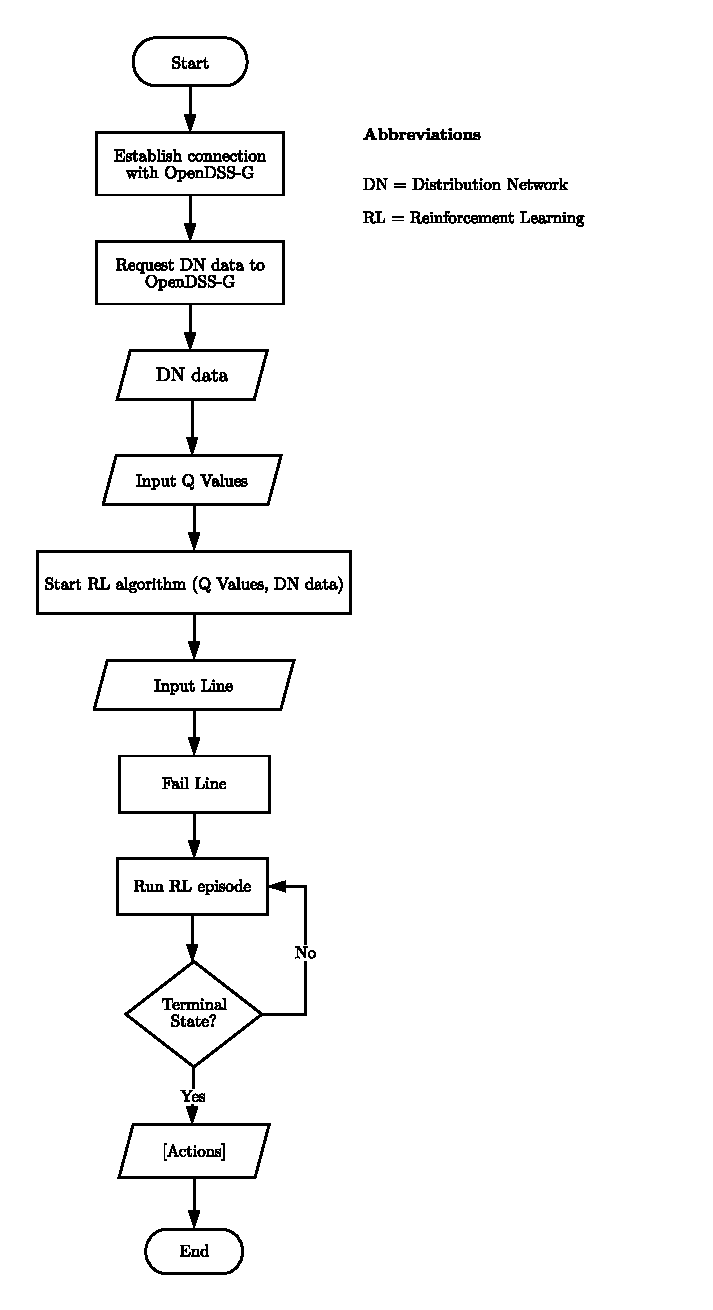
\includegraphics[scale=0.9]{_chapter1/fig/production_scenario.pdf}
    \caption{SR Algorithm - Production Scenario}
    \label{ch1:fig:production_blocks}
\end{figure}

Figure \ref{ch1:fig:production_blocks} shows that Production scenario behaves similarly to Training but with some exceptions. First, the initial 
connection is carried out with OpenDSS-G. Second, the Q Values matrix has been already computed, 
so this scenario aims to apply the Service Restoration plan to lead the network to the best possible 
state after a fault occurrence through self-healing. Third, RL episode runs only once and performs 
just the necessary switching operations until it reaches the terminal state, instead of switching 
operations for all possible faults and switch status combinations. And last, this results in a list 
of actions performed during the SR plan and an updated Q Values matrix. 